Nach dem Verknüpfen der Bilder verbleiben neben den Defekten noch schmale horizontale Streifen (vgl. Abbildung \ref{img:minAndMaxLink} und \ref{img:diffImage}).
Wenn man die beiden Kamerabilder mit phasenverschobenen Streifenmustern übereinanderlegt, bilden sich Überlappungen der Streifen.
Diese können durch eine Reihe von Ungenauigkeiten im gesamten Prozess entstehen.
Zum besseren Verständnis muss auf die Differenzen zwischen dem aufgenommenen Kamerabild und der erzeugten Muster auf dem Bildschirm eingegangen werden.

% Unterschiede zwischen Kameraufnahme und Monitorbild
{
	\FloatBarrier
    \subsection{Unterschiede zwischen Kameraufnahme und Monitorbild}
    \label{sub:unterschiedeKameraUndMonitor}
    Das Kameraobjektiv hat bestimmte Einstellungsmöglichkeiten, darunter die Blende und der Fokus.
Aufgrund der festen Brennweite des verwendeten Objektivs wird der Einfluss der Brennweite nicht genauer betrachtet.
Die entscheidenden Einstellungen für diesen Prozess sind also der Fokus und die Blende.
Über die Fokussteuerung kann eine einzelne Tiefenebene im Bild scharf gestellt werden.
Da das Prüfobjekt und das Streifenmuster in unterschiedlichen Tiefenebenen liegen, führt das bereits dazu, dass im Kamerabild nicht beides gleichzeitig fokussiert werden kann.
Der Fokus liegt zur Prüfung auf der Oberfläche des Objekts.
Dadurch wird das Streifenmuster unscharf, wodurch die Breiten der hellen und dunklen Streifen verändert werden.
Die zweite Einstellungsmöglichkeit ist die Blende.
Öffnet man diese weiter, lässt man mehr Licht in den Kamerasensor.
Durch mehr einfallendes Licht vergrößern sich die Breiten der hellen Streifen im Bild.
Oberflächendefekte des Prüfobjekts werden gleichzeitig besser sichtbar.
Zur Kompensation der unterschiedlichen Streifenbreiten im Kamerabild müssen die Breiten der hellen und dunklen Streifen im erzeugten Muster unterschiedlich gewählt werden (siehe Abbildung \ref{img:differenceCamPat}).

\begin{figure}[H]
	\centering
	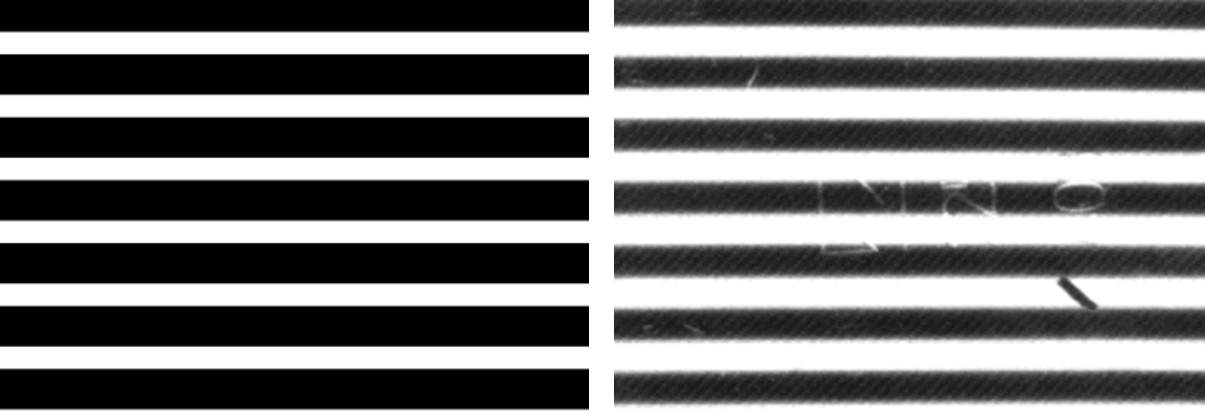
\includegraphics[width=\textwidth]{03_sichtpruefungDurchLichtstreuung/optimierungen/unterschiedeKameraUndMonitor/figures/differenceCameraPattern}
	\caption[Unterschied zwischen Muster und Kameraaufnahme]{Unterschied zwischen Muster und Kameraaufnahme. Links erzeugtes Muster mit fünf Pixel Breite der hellen und neun Pixel Breite der dunklen Streifen, Rechts Kameraaufnahme}
	\label{img:differenceCamPat}
\end{figure}

\noindent
Man muss also mit Streifenmustern arbeiten, die von der Gleichung \ref{eq:rstreifenmuster} abweichen und unterschiedliche Breiten für die hellen und dunklen Streifen haben.
Es kommt dazu, dass die hellen und dunklen Streifen im Kamerabild unter Umständen nicht exakt gleich breit sein können, da die Anpassung der Streifenbreiten lediglich auf pixelgenauer Ebene durchgeführt werden kann.
Außerdem gibt es auch bei der Phase der Streifenmuster die Beschränkung, dass die maximale Genauigkeit der Verschiebung auch ein Pixel beträgt.
Das bedeutet, dass die Streifen selbst bei exakt gleicher Breite unter dem Kamerabild nicht genau versetzt voneinander liegen.
Es kommt hinzu, dass diese Genauigkeit sich auf den projizierenden Bildschirm bezieht.
Durch das Brillenglas zwischen der Kamera und dem Bildschirm kann die Phasenverschiebung im Kamerabild also mit zusätzlichen Fehlern behaftet sein.
Außerdem ist zu beachten, dass in der Kameraaufnahme stets ein Rauschen die Szene überlagert.
}

% Muster mit unterschiedlichen Breiten Streifenbreiten
{
	\FloatBarrier
    \subsection{Muster mit unterschiedlichen Streifenbreiten}
    \label{sub:musterUnterschiedlichenStreifenbreiten}
    Das erzeugte Streifenmuster in Abbildung \ref{img:differenceCamPat} hat nicht mehr den Grauwertverlauf einer Rechteckschwingung (vgl. Abbildung \ref{tikz:abbRechteckschwingung}) entlang der Ausbreitungsrichtung.
Dadurch lässt sich das Streifenmuster nicht mehr in der Form aus Gleichung \ref{eq:rstreifenmuster} darstellen.
Der Grauwertverlauf in einer Zeile bzw. Spalte eines solchen Streifenmusters entspricht einer Impulsschwingung (siehe Abbildung \ref{tikz:abbPulsewave}).
%
% Abbildung: Pulswave
{
	\begin{figure}[H]
		\centering
		\begin{adjustbox}{width=\textwidth}
	\begin{tikzpicture}
	
		% Koordinatensystem
		\draw[thick,-stealth,black] (0,0)--(16,0) node[below] {$x$};
		\draw[thick,-stealth,black] (0,0)--(0,4.25) node[left] {$m_1(x,y_0)$};
		\draw[thick,black] (0,0) -- (0,-0.1) node[anchor=north,fill=white] {$0$};
		\draw[thick,black] (15,0) -- (15,-0.1) node[anchor=north,fill=white] {\acrshort{lwidth}};
		\draw[thick,black] (0,0) -- (-0.1,0) node[anchor=east,fill=white] {$0$};
		\draw[thick,black] (0,3.75) -- (-0.1,3.75) node[anchor=east,fill=white] {$255$};

		% Funktion, erste Periode
		\draw[blue, thick] (0,3.75) -- (1,3.75);
		\draw[blue, thick] (1,3.75) -- (1,0);
		\draw[blue, thick] (1,0) -- (3.75,0);
		\draw[blue, thick] (3.75,0) -- (3.75,3.75);
		
		% Funktion, zweite Periode
		\draw[blue, thick] (3.75,3.75) -- (4.75,3.75);
		\draw[blue, thick] (4.75,3.75) -- (4.75,0);
		\draw[blue, thick] (4.75,0) -- (7.5,0);
		\draw[blue, thick] (7.5,0) -- (7.5,3.75);
		
		% Funktion, dritte Periode
		\draw[blue, thick] (7.5,3.75) -- (8.5,3.75);
		\draw[blue, thick] (8.5,3.75) -- (8.5,0);
		\draw[blue, thick] (8.5,0) -- (11.25,0);
		\draw[blue, thick] (11.25,0) -- (11.25,3.75);
		
		% Funktion, vierte Periode
		\draw[blue, thick] (11.25,3.75) -- (12.25,3.75);
		\draw[blue, thick] (12.25,3.75) -- (12.25,0);
		\draw[blue, thick] (12.25,0) -- (15,0);

		\end{tikzpicture}
\end{adjustbox}
\caption[Impulsschwingung bzw. \textit{eng: pulse wave, rectangular wave}]{Impulsschwingung, \textit{eng: pulse wave, rectangular wave}, eines Streifenmusters mit Ausbreitungsrichtung in $x$ bei fester, aber beliebiger Zeile $y_0$.}
		\label{tikz:abbPulsewave}
	\end{figure}
}
%
\noindent
Um eine Gleichung für eine solche Impulsschwingung (siehe Abbildung \ref{tikz:abbPulsewave}) herzuleiten, kann man die periodische Sägezahnschwingung verwenden \cite{waveGeneration}.
Eine Sägezahnschwingung lässt sich darstellen durch (vgl. \cite{sawtoothWave}):
%
\begin{equation} \label{eq:saegezahnschwingung}
	w_f(t) = 2 \left( ft - \left\lfloor ft \right\rfloor \right) - 1
\end{equation}
%
\noindent
$f$ bezeichnet die Frequenz der Sägezahnschwingung und steht analog zu Gleichung \ref{eq:einheitsrechteckschwingung} über den Kehrwert im Zusammenhang mit der Periodenlänge der Sägezahnschwingung $w_f(t)$:
%
\begin{equation*}
	f = \dfrac{1}{T}
\end{equation*}
%
Mit $T = 3$ erhält man folgendes Schaubild (siehe Abbildung \ref{tikz:abbsaegezahnSchwingung}).
%
% Abbildung: Sägezahnschwingung
{
	\begin{figure}[H]
		\centering
		\input{03_sichtpruefungDurchLichtstreuung/optimierungen/musterMitUnterschiedlichenStreifenbreiten/figures/abbSaegezahnSchwingung}
		\label{tikz:abbsaegezahnSchwingung}
	\end{figure}
}
%
\noindent
Bildet man die Differenz von zwei zueinander um $\tfrac{D}{f}$  in $t$-Richtung versetzten Sä\-ge\-zahn\-funk\-ti\-onen, erhält man die Impulsschwingung $p_{f,D}(t)$:
%
\begin{equation} \label{eq:pulsewave}
	p_{f,D}(t) = w_f(t - \dfrac{D}{f}) - w_f(t) - w_f(- \dfrac{D}{f}),
	\quad
	D \in \left(0,1\right] \subset \acrshortmath{real}
\end{equation}
%
\noindent
$D$ wird Tastgrad (\textit{engl: duty cycle}) genannt und bezeichnet die Impulsdauer der Impulsschwingung im Verhältnis zur Periodenlänge $T$.
Auch für die Impulsschwingung gilt der Zusammenhang zwischen der Frequenz $f$ und der Periodendauer $T$ wie für die Sä\-ge\-zahn\-schwin\-gung:
%
\begin{equation*}
	f = \dfrac{1}{T}
\end{equation*}
%
Somit erhält man mit $D = \tfrac{1}{2}$ eine Rechteckschwingung wie auch in Abbildung \ref{tikz:abbRechteckschwingung}.
Ein Schaubild der Gleichung \ref{eq:pulsewave} wird in Abbildung \ref{tikz:abbNormalPulsewave} dargestellt.
%
% Abbildung: Normale Impulsschwingung
{
	\begin{figure}[H]
		\centering
		\begin{adjustbox}{width=\textwidth}
	\begin{tikzpicture}[declare function={sawtooth(\x) = 1.5*(2*((\x/3)-0.5-floor((\x/3))));}]
	
		% Koordinatensystem
		\draw[thick,-stealth,black] (-8,0)--(8,0) node[below] {$t$};
		\draw[thick,-stealth,black] (0,-2.125)--(0,2.125) node[left] {$p_{\tfrac{1}{3},\tfrac{1}{3}}(t)$};
		
		% Funktion
		\draw[name path = func1, blue, thick, domain=-8:8, samples=600] plot (\x, {sawtooth(\x - (1/3) * 3) - sawtooth(\x) - sawtooth(-(1/3) * 3)});
		
		% Achsenbeschriftungen
		\draw[thick,black] (0,-1.5) -- (-0.1,-1.5) node[anchor=east,fill=white] {$-1$};
		\draw[thick,black] (0,1.5) -- (-0.1,1.5) node[anchor=east,fill=white] {$1$};
		\draw[thick,black] (-7,0) -- (-7,-0.1) node[anchor=north,fill=white] {$-7$};
		\draw[thick,black] (-6,0) -- (-6,-0.1) node[anchor=north,fill=white] {$-6$};
		\draw[thick,black] (-5,0) -- (-5,-0.1) node[anchor=north,fill=white] {$-5$};
		\draw[thick,black] (-4,0) -- (-4,-0.1) node[anchor=north,fill=white] {$-4$};
		\draw[thick,black] (-3,0) -- (-3,-0.1) node[anchor=north,fill=white] {$-3$};
		\draw[thick,black] (-2,0) -- (-2,-0.1) node[anchor=north,fill=white] {$-2$};
		\draw[thick,black] (-1,0) -- (-1,-0.1) node[anchor=north,fill=white] {$-1$};
		\draw[thick,black] (1,0) -- (1,-0.1) node[anchor=north,fill=white] {$1$};
		\draw[thick,black] (2,0) -- (2,-0.1) node[anchor=north,fill=white] {$2$};
		\draw[thick,black] (3,0) -- (3,-0.1) node[anchor=north,fill=white] {$3$};
		\draw[thick,black] (4,0) -- (4,-0.1) node[anchor=north,fill=white] {$4$};
		\draw[thick,black] (5,0) -- (5,-0.1) node[anchor=north,fill=white] {$5$};
		\draw[thick,black] (6,0) -- (6,-0.1) node[anchor=north,fill=white] {$6$};
		\draw[thick,black] (7,0) -- (7,-0.1) node[anchor=north,fill=white] {$7$};	
		
	\end{tikzpicture}
\end{adjustbox}
\caption[Einheits-Impulsschwingung]{Einheits-Impulsschwingung nach Gleichung \ref{eq:pulsewave} mit $f = \tfrac{1}{3}$ und $D = \tfrac{1}{3}$.}
		\label{tikz:abbNormalPulsewave}
	\end{figure}
}
%
\noindent
Aus Gleichung \ref{eq:pulsewave} lässt sich somit eine mathematische Darstellung für Streifenmuster mit unterschiedlichen Streifenbreiten aufschreiben:
%
\begin{equation} \label{eq:impulsStreifenmuster}
	\begin{gathered}
		m_k(x,y) = A_m \left( 1 + p_{f,D}\left( x - \dfrac{1}{2 \pi f} \psi_k \right) \right),
		\\
		f = \dfrac{N_p}{\acrshortmath{lwidth}},
		\quad
		D \in \left(0,1\right] \subset \acrshortmath{real},
		\quad
		\psi_k = (k - 1)\dfrac{2\pi}{N_{shift}},
		\quad
		k \in \lbrace 1,\ldots,N_{shift}\rbrace
	\end{gathered}
\end{equation}
%
Wie auch in Gleichung \ref{eq:rstreifenmuster} gilt für dieses Muster die Periodizität in der Ausbreitungsrichtung.
Auch hier bezeichnet $A_m$ die Amplitude, $N_p$ die Anzahl der Perioden über die Monitorbreite \acrshort{lwidth}, $N_{shift}$ die Anzahl der Phasenverschiebungen und $\psi_k$ die Phasenverschiebung des $k$-ten Musters.
Zusätzlich zu diesen Parametern hat man den Tastgrad $D$, der in diesem Fall die Breite der hellen Streifen im Verhältnis zu der Periodenlänge $T$ angibt.
Die Periodenlänge $T$ ist im Streifenmuster die Summe der Breite eines einzelnen dunklen und eines einzelnen hellen Streifens.
Analog zu Gleichung \ref{eq:impulsStreifenmuster} lässt sich auch ein horizontales Streifenmuster mit Ausbreitungsrichtung in $y$ über die Monitorhöhe \acrshort{lheight} beschreiben.
Das Bild eines horizontalen Streifenmusters analog zu Gleichung \ref{eq:impulsStreifenmuster}, d. h. mit Ausbreitungsrichtung in $y$, wird in Abbildung \ref{tikz:abbImpulsStreifenmuster} dargestellt.
%
% Abbildung: Impuls-Streifenmuster
{
	\begin{figure}[H]
		\centering
		\begin{adjustbox}{width=\textwidth}
	\begin{tikzpicture}[every node/.style={inner sep=0,outer sep=0}]
	
		\node [anchor=north east] (img1) at (-0.03\textwidth,0) {
\includegraphics[frame,width=.47\textwidth]{03_sichtpruefungDurchLichtstreuung/optimierungen/musterMitUnterschiedlichenStreifenbreiten/figures/impulsStreifenmuster}};
		\node [below=0.2cm of img1] {Muster $m_1$ mit $\psi_1 = 0$};
		\node [anchor=north west] (img2) at (0.03\textwidth,0) {
\includegraphics[frame,width=.47\textwidth]{03_sichtpruefungDurchLichtstreuung/optimierungen/musterMitUnterschiedlichenStreifenbreiten/figures/impulsStreifenmuster_shifted}};
		\node [below=0.2cm of img2] {Muster $m_3$ mit $\psi_3 = \pi$};
		
	\end{tikzpicture}
\end{adjustbox}
\caption[Streifenmuster durch Impulsschwingung]{Horizontale Streifenmuster analog zu Gleichung \ref{eq:impulsStreifenmuster} erzeugt, mit $A_m = 127.5$, $N_p = 4$, $\acrshortmath{lheight} = 272$, $N_{shift} = 4$ und $D = \tfrac{1}{4}$. Die hellen Streifen haben damit eine Höhe von 17 Pixeln und die dunklen Streifen eine Höhe von 51 Pixeln.}
		\label{tikz:abbImpulsStreifenmuster}
	\end{figure}
}
}

% Verknüpfung von mehreren Kameraaufnahmen
{
	\FloatBarrier
    \subsection{Verknüpfung von mehreren Kameraaufnahmen}
    \label{sub:verknuepfungMehrererKameraaufnahmen}
    Da die Kameraeinstellungen auf die Prüfstation und Prüfbedingungen angepasst werden müssen, sind die Möglichkeiten zur Eliminierung der Streifen im Vorhinein begrenzt.
Die Nachbearbeitung kann über verschiedene Ansätze erfolgen.
Aufgrund der Periodizität und der festen Ausbreitungsrichtung der Streifen bietet es sich an, die Fourier-Analyse anzuwenden.
Man untersucht die Frequenzkomponenten der Streifen und filtert speziell diese aus dem Bild heraus, um sie zu entfernen.
Diese Methode kann allerdings nicht die fehlende Information an den dunklen Streifen wiederherstellen, sondern lediglich eine Bildverbesserung durchführen.
Eine andere Möglichkeit ist das Hinzuziehen von weiteren Bildern.
Da an den Stellen der horizontalen Streifen die Information fehlt, kann man zusätzliche Muster zur Hand nehmen, um die Informationen zu ergänzen.
Man zieht weitere phasenverschobene Muster hinzu, sodass man eine gerade Anzahl an Phasenverschiebungen hat.
Daraus kann man die Informationen vereinen und eliminiert die Streifen, welche durch Überlappungen der versetzen Streifen in den Kamerabildern entstehen.
Im Folgenden werden als Beispiel die vier Kamerabilder der Streifenmustern $m_1 - m_4$ miteinander verknüpft, die mit $N_{shift} = 4$ gebildet wurden.
Aus den vier aufgenommenen Bildern verknüpft man je zwei Bilder mit der betragsmäßigen Differenz, in denen die Streifenmuster eine Phasenverschiebung von $\pi$ zueinander haben.
Die zwei resultierenden Bilder haben zueinander versetzte Streifen, die aus den Überlappungen entstehen.
Zum Schluss kann man die beiden Bilder so verknüpfen, dass man stets den Bildpunkt mit dem höheren Helligkeitswert nimmt.
Das entspricht der Maximierung.
Analog kann man auch die horizontalen Streifen aus Abbildung \ref{img:minAndMaxLink} eliminieren, in welcher die Typen von Fehlstellen isoliert voneinander betrachtet wurden.
In Abbildung \ref{img:imageTree} werden die einzelnen Schritte dieses Verfahrens veranschaulicht.
Analog lässt sich auch die Verknüpfung von mehr als vier phasenverschobenen Streifenmustern durchführen.

\begin{figure}[H]
	\centering
	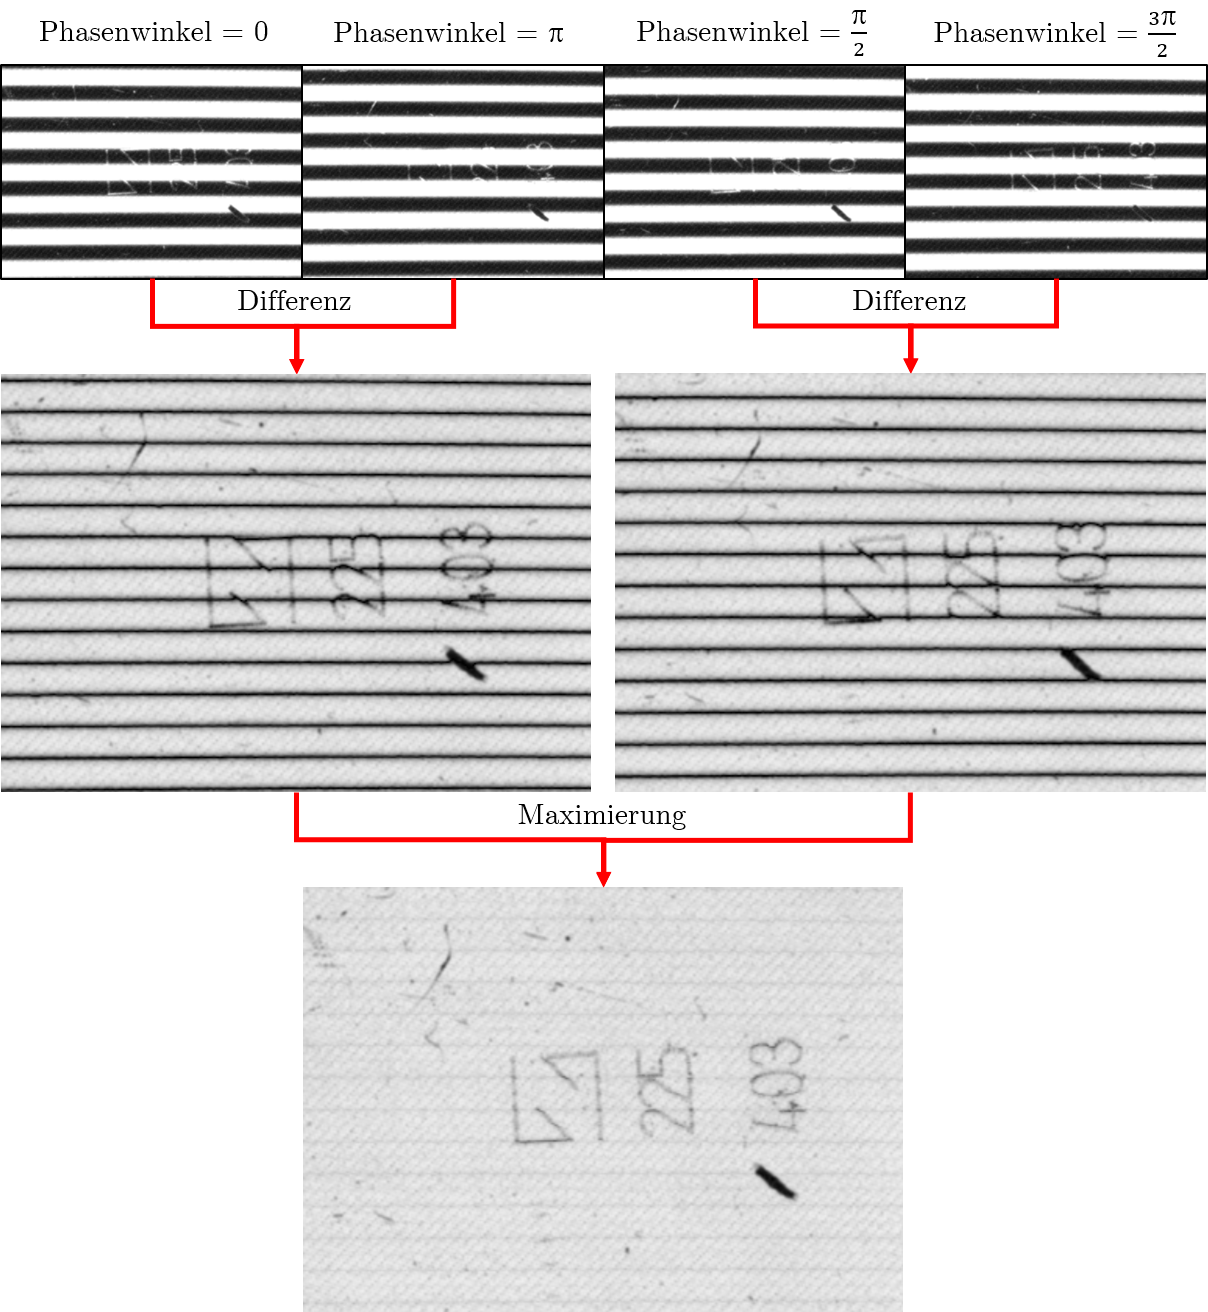
\includegraphics[width=\textwidth]{03_sichtpruefungDurchLichtstreuung/optimierungen/figures/imageTree}
	\caption[Prozess der Hervorhebung von Oberflächendefekten]{Prozess zur Hervorhebung von Oberflächendefekten mit $N_{shift} = 4$.}
	\label{img:imageTree}
\end{figure}
}

% Nachbearbeitung mit der Fourier-Analyse
{
	\FloatBarrier
    \subsection{Nachbearbeitung mit der Fourier-Analyse}
    \label{sub:nachbearbeitungFourierAnalyse}
    \noindent
Im praktischen Durchlauf verbleiben auch im letzten Bild noch sehr schwache horizontale Streifen.
Das liegt an den oben genannten Ungenauigkeiten im Prüfprozess und der Mustererzeugung.
Da das Ergebnis mit weiteren phasenverschobenen Streifenmustern stetig besser wird, könnte man diese durch eine höhere Anzahl von Streifenmustern $N_{shift}$ eliminieren.
Dabei gilt zu beachten, dass man im Diskreten arbeitet und bei einer sehr hohen Anzahl von Phasenverschiebungen Messfehler und Gleitpunktfehler zum Tragen kommen.
Das bedeutet, man muss eine zum Prüfaufbau passende Anzahl an Mustern verwenden, um bessere Ergebnisse dokumentieren zu können.
Zur Bildverbesserung hat man aber auch die Möglichkeit, die zuvor erwähnte Fourier-Analyse anzuwenden.
Die noch verbliebenen Strukturen lassen sich im Amplitudenspektrum des Bildes durch die Ausbreitungsrichtung finden.
Da diese Strukturen nur noch sehr schwach im Bild vorhanden ist, sind die jeweiligen Frequenzkomponenten auch dementsprechend gering gewichtet (siehe Abbildung \ref{img:amplitudeSpectrum}).

\begin{figure}[H]
	\centering
	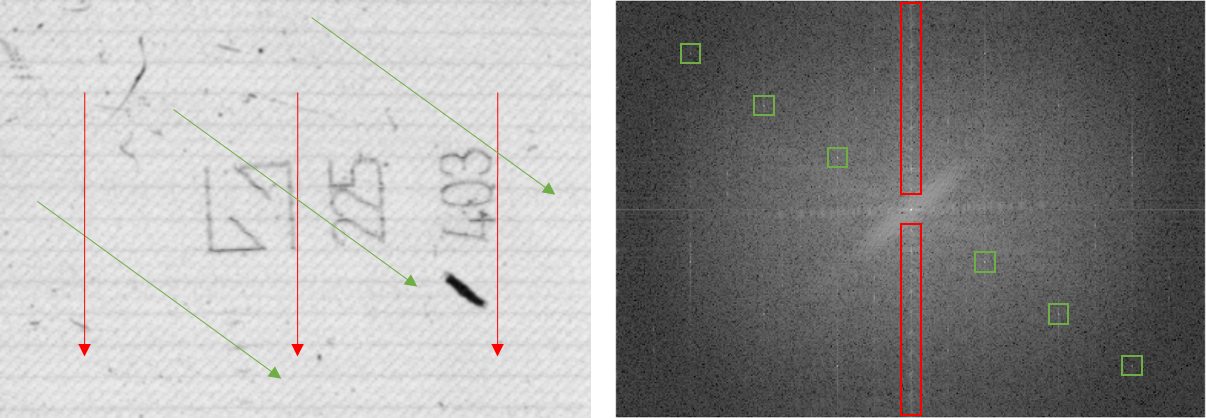
\includegraphics[width=\textwidth]{03_sichtpruefungDurchLichtstreuung/optimierungen/figures/amplitudeSpectrum}
	\caption[Amplitudenspektrum des Gesamtbildes]{Amplitudenspektrum des Gesamtbildes. (mit Markierungen)}
	\label{img:amplitudeSpectrum}
\end{figure}

\noindent
In Rot ist im Bild die Ausbreitungsrichtung der ersten Struktur markiert, die entsprechenden Gewichte der Frequenzkomponenten sind in derselben Farbe im Amplitudenspektrum gezeichnet.
Analog sind in Grün die für die zweite Struktur relevante Ausbreitungsrichtung und Gewichte der Frequenzkomponenten markiert.
Filtert man im Amplitudenspektrum die markierten Bereiche heraus und wendet die inverse Fourier-Transformation an, erhält man ein Bild, indem die beiden störenden Strukturen nicht mehr vorhanden sind.
Das Ergebnisbild wird durch ein geeignetes Online-Werkzeug \cite{fourierTool} berechnet und in Abbildung \ref{img:frequencyFiltered} dargestellt.

\begin{figure}[H]
	\centering
	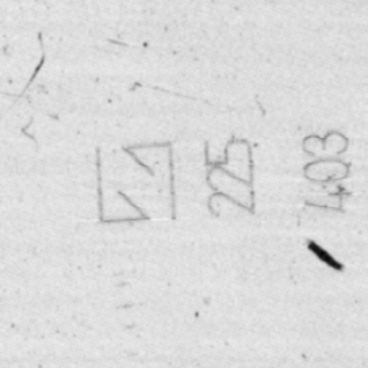
\includegraphics[width=0.4\textwidth]{03_sichtpruefungDurchLichtstreuung/optimierungen/figures/frequencyFiltered}
	\caption[Bild mit angewandtem frequenzselektives Filter]{Angewandtes frequenzselektives Filter nach Abbildung \ref{img:amplitudeSpectrum}. Erstellt mit dem Online-Werkzeug \glqq Fourifier\grqq ~von © 2020 Ejectamenta.\cite{fourierTool}\footnotemark}
	\label{img:frequencyFiltered}
\end{figure}
\footnotetext{Anmerkungen: Das Bild musste aufgrund der Anforderungen des verwendeten Online-Werkzeugs zugeschnitten werden. Außerdem wurden die Frequenzkomponenten \glqq händisch\grqq ~entfernt, weshalb das Bild fehlerbehaftet ist. Das Bild konnte auch nicht auf Korrektheit geprüft werden und dient nur der Veranschaulichung. Die Nutzungsrechte unterliegen der Lizenz von © 2020 Ejectamenta. Für weitere Informationen zu Geschäfts- und Nutzungsbedingungen siehe: \url{https://ejectamenta.com/about/terms-of-service/}}
}

\noindent
Mit dem vorgestellten deflektometrischen Verfahren wurden Oberflächen\-de\-fekte wie z. B. Kratzer, Eingravierungen oder Partikel auf transparenten und spiegelnden Prüfobjekten sichtbar gemacht.
Das erzeugte Gesamtbild dieses Verfahrens kann nun durch anschließende Bildverarbeitung analysiert und geprüft werden.
In diesem konkreten Fall würden sich z. B. Kratzer detektieren oder die eingravierten Zeichen auslesen lassen.

\p
Dieses Verfahren kann je nach Parametrisierung mit unterschiedlicher Empfindlichkeit Abweichungen in der Oberfläche sichtbar machen, die die Lichtreflexionen beeinflussen.
Dadurch eignet es sich besonders für Brillengläser und transparente Objekte.